\section{Introduction}
\label{sec:intro}

%% datacenter is high impact topic 
Data centers (DCs) are a critical piece of today's computing
infrastructure that drive key networked applications~\cite{}. The key
benefits offered by these large-scale consolidated computing power
are: the economies of scale, reduced or amortized management costs,
better utilization of hardware, and \blue{the ability to dynamically
  scale applications in response to changing workload patterns.}


%
%% datacenter network needs to be designed carefully
The key component that drives the success of such large-scale
datacenters is an efficient, robust, and cost-effective {\em network
  fabric}. In particular, the data center network designs must satisfy
several potentially conflicting goals: high performance (e.g., high
throughput and low latency)~\cite{fattree,vl2}; low equipment and
management cost~\cite{fattree,popa-cost}; robustness to extremely
dynamic traffic patterns~\cite{proteus,3db,flyways,cthru}; incremental
expandability to add new servers or racks~\cite{legup,jellyfish}; and
a host of other practical concerns including cabling complexity,
power, and cooling~\cite{farrington,portland,cabling}.



%%% taxonomy of prior work
The traditional data center architectures have been fixed (wired) in
their design. Hence, due to the highly variable and unpredictable
nature of data center workloads~\cite{vl2}, these traditional fixed
designs either (a) offer poor performance at low cost (e.g., simple
trees or leaf/spine architectures), or (b) are over-provisioned (e.g.,
fat-tree architectures) to account for the {\em worst-case}
communication requirements; over-provisioning results in higher cost
and maintenance of networking architecture.
%
Some recent works augment the simple wired infrastructure with
additional inter-rack wireless~\cite{flyways,3db} or optical
links~\cite{cthru} to impart certain flexibility to the network
architectures and thus help alleviate congested hotspots.


%Our overall vision with figure
%However, the overall vision of a fully wireless and a highly
%flexibible data center network architecture with \blue{very favorable}
%cost-performance tradeoff remains far from realized. The goal of our
%research proposal is to realize this vision.
\mypara{Our vision}
We take the flexibility offered by wireless
inter-rack links to the logical extreme and propose to design an
\emph{all-wireless inter-rack data center fabric}. Our vision, if
realized, would provide unprecedented degrees of flexibility for data
centers. That is, it will allow operators to dynamically reconfigure
the {\em entire} network topology to adapt to changing traffic
demands. Moreover, a wireless architecture eliminates maintenance and
operational costs due to cabling complexities~\cite{hp-cable}, and
more importantly, can \blue{facilitate} topology structures that would
otherwise remain ``paper designs'' due to the perceived cabling
complexity.


\begin{wrapfigure}{r}{0.5\textwidth}
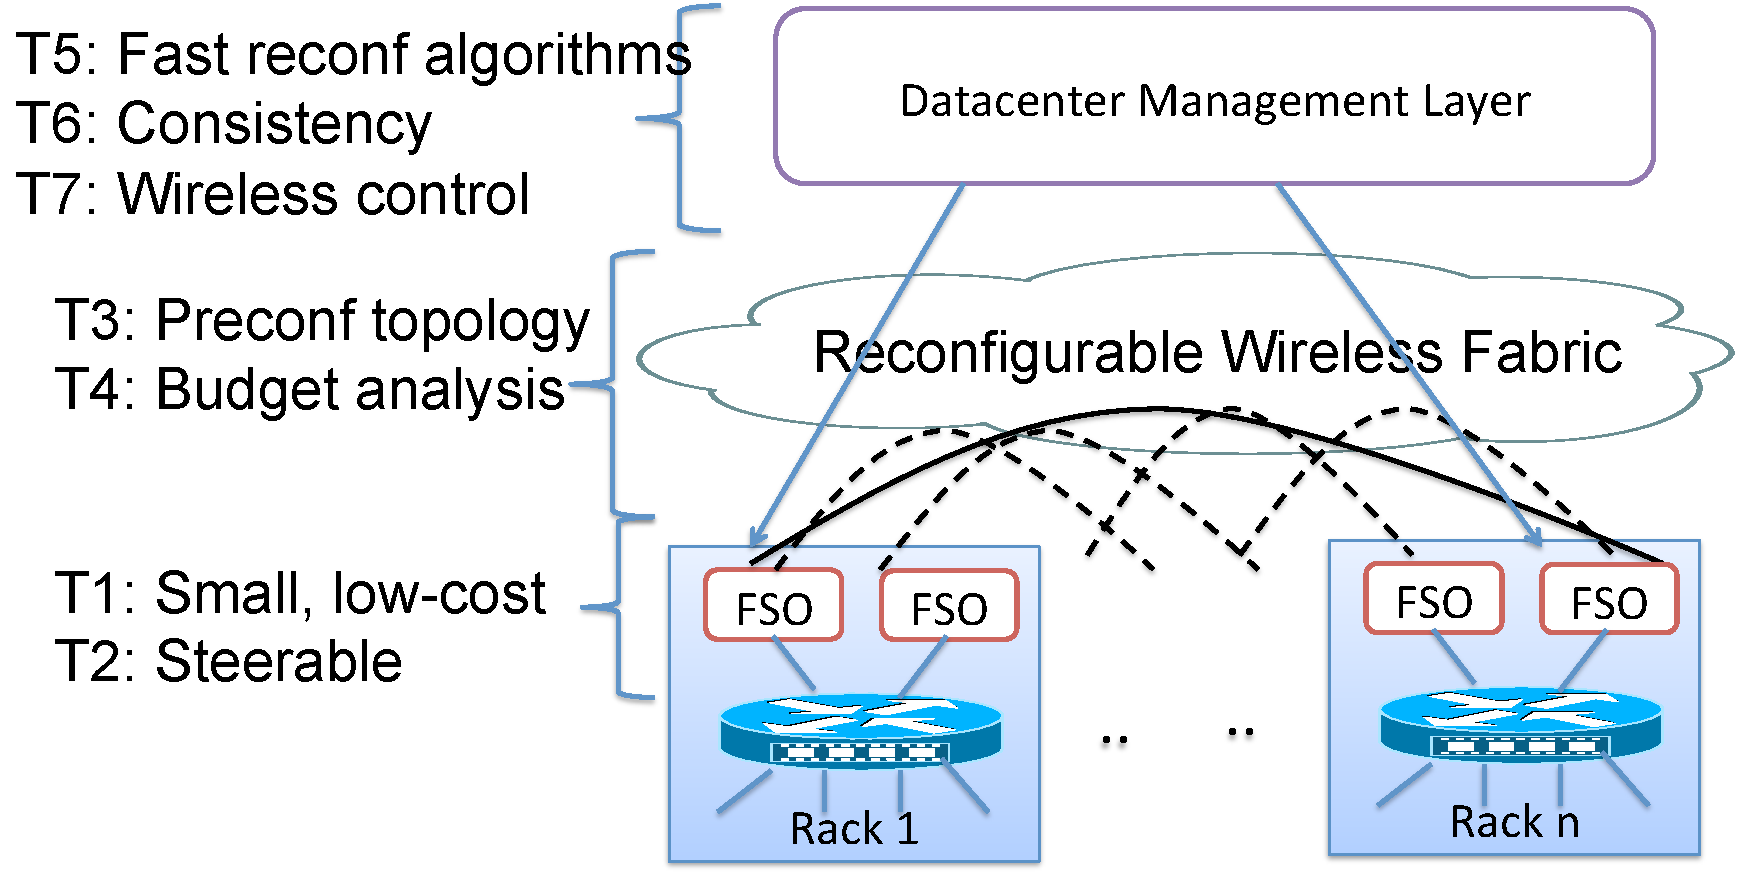
\includegraphics[width=220pt]{PPTFigs/introview_temp.pdf}
\caption{Overview of the \ArchName vision}
\label{fig:vision}
\end{wrapfigure}



To realize our vision of an \emph{all-wireless} inter-rack data center
fabric, we look beyond the traditional \blue{radio-frequency (RF)
  based (e.g., 60GHz)} solutions and explore a somewhat non-standard
``wireless'' technology, namely {\em Free-Space Optics} (FSO).  FSO
uses visible or infra-red lasers to implement point-to-point data
links, and offers very high data rates ($>$1~Gbps) at long ranges,
\blue{even with minimal transmission power.}  \blue{Most importantly},
unlike the RF wireless technologies, FSO communication links have a
minimal wireless-interference footprint (due to their low wavelength)
and their usage is not constrained by federal regulations.


\mypara{Research plan and Intellectual Merit}
%
While FSO is an enabling technology, there are various scientific
challenges that need to be addressed before we can realize a
\blue{viable fully-flexible} DC network fabric. Our research proposal
plans to address these challenges and build an FSO-based DC network
prototype. \blue{We start with motivating our vision, and presenting
  our overall network architecture and its key challenges in the
  following section.}

\begin{packeditemize}

\item Developing cost-effective, small-form factor (\taskref{task:fso:sfp}) and
rapidly steerable Free-Space Optical links  (\taskref{task:fso:steer}); 

\item Algorithmic foundations for flexible topology design subject to physical
and geometric constraints (\taskref{task:topology})

\item System challenges in design of fast reconfiguration algorithms
(\taskref{task:system:fastalgo}, consistency mechanisms
(\taskref{task:system:dataplane}), and eliminating the need for wired
out-of-band control (\taskref{task:system:ctrlchannel})
 

\item Proof-of-concept testbed

\end{packeditemize}



\para{Team Qualifications}   Our proposed research requires a collaborative
effort that spans aspects of optical technologies, algorithmic foundations, and
networked systems design. Our team comprises three computer scientists and one
mechanical engineer  with complementary  expertise spanning the domains of
wireless networking~\cite{}, network management~\cite{}, software-defined
networking~\cite{}, and the use of laser-based optical technologies~\cite{}. 

%mechanical engineer with expertise in laser-based optical measurement
%techniques, giving us a complete spectrum of expertise needed for
%various scientific aspects of our research proposal.

\eat{
\para{Proposal Objectives, and Our Team.}  To the context of the above
vision of an FSO-based inter-rack fabric for a data center, our
proposal has the following specific objectives.

\begin{itemize}
\item
We will design an FSO communication device that is cost-effective and
has a small-form factor, for use in a data center network. The device
will include an appropriate steering and alignment mechanism with
effective speed and precision; we will explore feasibility of two
possible steering mechanisms in our research. {\bf See Section~\ref{sec:fso}}.

\item
We will design efficient algorithms for two topology design problems
that arise in our context, viz., (a) Pre-configured Topology design,
i.e., determination of initial alignment/configuration of the FSO
devices, under various design constraints and available traffic
statistics, and (b) Reconfiguration strategy, which controls the
real-time configuration of FSO devices based on the current network
traffic. {\bf See Section~\ref{sec:top}}.

\item
We will address various network management challenges that arise in
our context. In particular, $\ldots$ {\bf See Section~\ref{sec:system}}.

\item
We will build a prototype of an FSO device, develop a system prototype
over XX platform, and conduct extensive simulations over real data
center traffic to demonstrate viability and performance of our overall
vision. {\bf See Section~\ref{sec:prototype}}.
\end{itemize}
}

